\documentclass[conference]{IEEEtran}
\usepackage{graphicx}
\usepackage{booktabs}
\usepackage{amsmath}
\usepackage{array}
\usepackage{url}
\usepackage[hidelinks]{hyperref}
\graphicspath{{figures/}{../results/}}
\title{Evidence-Grounded Prompting and Abstention in Biomedical Question Answering: A Reproducible PubMedQA Case Study}
\author{\IEEEauthorblockN{Aditya Mohan Saha}\IEEEauthorblockA{MCL2026001\\Indian Institute of Information Technology, Allahabad}}
\begin{document}
\maketitle
\begin{abstract}
Factual reliability of language models is not fully described by a single accuracy figure: generated decisions may depend on access to evidence, the evaluation unit, and whether a model can decline to answer. We present a controlled case study on the expert-labeled PubMedQA dataset using the open-weight Qwen2.5-0.5B-Instruct checkpoint. We compare a development-set majority predictor with three fixed-model prompting conditions: question only, question with the associated abstract, and question with the abstract plus permission to abstain. An executed Google Colab run produced 800 archived predictions across four conditions on the same 200 held-out questions. Question-only, abstract, and abstract-plus-abstention accuracies were 11.0\%, 17.5\%, and 20.5\%, respectively; the majority predictor achieved 55.0\%. The corresponding macro-F1 scores were 0.0664, 0.1476, 0.1715, and 0.2366 for the majority baseline. Adding context recovered 19 previously wrong decisions but lost six previously correct decisions. Crucially, all model conditions had zero recall for the \texttt{no} class, and the abstention-enabled condition produced no abstentions. An independent audit of archived responses reproduces the summary statistics. The results support a narrow finding that supplied abstract context improved label agreement in this setting, while revealing severe label-selection failure and no demonstrated benefit from selective answering.
\end{abstract}
\begin{IEEEkeywords}
scientific factuality, PubMedQA, biomedical question answering, evidence grounding, large language models, abstention, reproducibility
\end{IEEEkeywords}

\section{Introduction}
Scientific use of large language models requires more than fluent prose. A response may assert a plausible conclusion without the evidence needed to substantiate it, cite an unsuitable source, or give a correct-looking answer for an incorrect reason. These problems are particularly salient in biomedical questions, where the interpretation of a study may depend on details of its population, design, measurements, and conclusions. The preceding literature review for this project organized scientific factuality into claim accuracy, evidence support, reasoning consistency, and domain validity. These dimensions motivate experiments that isolate an evaluation question instead of treating any single benchmark score as a universal factuality measure.

This paper studies one deliberately restricted aspect: agreement with expert-annotated \texttt{yes}, \texttt{no}, or \texttt{maybe} decisions on PubMedQA \cite{pubmedqa}. It does not ask a model to produce an evidence-cited scientific narrative or to score individual atomic claims. The question is whether the same pretrained instruction model changes its decisions when the associated abstract is supplied, and whether an explicit instruction permitting abstention causes it to withhold uncertain judgments. Both comparisons are possible without training a new large model or purchasing inference access.

The constrained setting is useful for two reasons. First, changing the prompt while keeping the checkpoint, held-out questions, decoding parameters, and parser fixed makes the resulting comparisons interpretable as \emph{within-study differences}. Second, it permits direct examination of misleading aggregate performance: a classifier that predicts only one answer class can appear somewhat successful on that class while failing elsewhere. A development-set majority predictor supplies a simple reference that prevents improvements within weak LLM configurations from being mistaken for adequate task performance.

The contribution of this work is therefore a reproducible teaching-scale controlled study, not a new model or a claimed first result. It includes a public dataset, one accessible compact checkpoint, saved item-level predictions, classwise and paired error analysis, a computational cost record, and an independent audit that does not require rerunning GPU inference. The comparison uses \emph{dataset-supplied evidence}. It is not a retrieval-augmented generation system, because no independent retriever selects or ranks documents.

\section{Background and Relationship to Prior Work}
\subsection{Biomedical decision benchmarks}
PubMedQA is a benchmark of biomedical research questions paired with the corresponding article's abstract context and an answer in the set \{\texttt{yes},\texttt{no},\texttt{maybe}\} \cite{pubmedqa}. The original dataset includes 1,000 expert-annotated instances, together with additional unlabeled and automatically generated material. In the task formulation, context is derived from the abstract while the long-answer field contains its conclusion. That distinction matters here: providing the conclusion as prompt input would be a different and potentially trivial task. This study therefore constructs the prompt from the question and the dataset's \texttt{CONTEXTS} field only.

A three-label classification benchmark gives a standardized outcome, but it does not tell us whether an explanation is scientifically sound, whether each proposition is supported, or whether a citation is accurate. A model could select the right label through memorization or a spurious shortcut. For this reason, all results below are described as \emph{benchmark decision agreement}, not as verified scientific reasoning or medical decision safety.

\subsection{Granularity, evidence and verification}
FActScore decomposes long-form generation into atomic claims and estimates the proportion supported by evidence \cite{factscore}. FELM instead annotates coherent response segments and accompanying factual error information across several settings \cite{felm}. ALCE evaluates cited text generation by considering answer correctness, fluency, and citation quality \cite{alce}. These studies illustrate different units of evaluation. Their metrics cannot simply be substituted for a short-label PubMedQA score, even though they share the wider goal of evaluating factuality.

The literature review also identifies evaluator reliability, temporal validity and cross-domain comparisons as outstanding concerns. Those problems exceed the resources and output format of the present experiment. A narrow question about a small model on one biomedical dataset is more defensible than claiming to have solved cross-domain factuality benchmarking without aligning tasks, evaluators and evidence sources.

\subsection{Abstention is not the \texttt{maybe} class}
The answer \texttt{maybe} belongs to the ground-truth PubMedQA taxonomy: it may express an uncertain or mixed scientific conclusion. By contrast, \texttt{abstain} in the present experiment is an additional response indicating that the system declines to provide a benchmark label. Treating \texttt{maybe} as an abstention would conflate the target class with system-level uncertainty. We therefore separately measure valid-label coverage and abstention frequency and count an abstention as incorrect for unconditional classification accuracy.

\section{Research Questions and Study Design}
The primary research question (RQ1) is: \emph{For Qwen2.5-0.5B-Instruct on a fixed set of expert-labeled PubMedQA questions, how does supplying the associated abstract change accuracy and macro-F1 relative to question-only prompting?} A positive net accuracy difference requires the abstract condition to correct more questions than it causes to become wrong. Because answer classes are imbalanced, per-class recall and macro-F1 are also necessary to understand which judgments change.

The secondary question (RQ2) is: \emph{When an abstention option is added to the evidence-grounded prompt, how do valid-answer coverage and accuracy among answered questions change?} A genuine selective-answering trade-off would require one or more \texttt{abstain} outputs, not merely different class predictions. The study has no expectation that either intervention must succeed.

The experimental pathway is a controlled comparison rather than reproduction of the original PubMedQA authors' trained benchmark model. Four conditions are evaluated: (i) a simple development-set majority predictor; (ii) a \emph{direct} prompt containing only the question; (iii) a \emph{context} prompt with the question and corresponding abstract; and (iv) \emph{context+abstain}, which adds permission to withhold an answer. The last three share the same checkpoint, input ordering, response format requirement, and generation settings. The prompt variants modify only the information or instruction being tested.

\section{Dataset and Preprocessing}
\subsection{Source and retained split}
The executed notebook downloaded the official \texttt{ori\_pqal.json} file from the PubMedQA repository and recorded its SHA-256 digest. It validated a dictionary of 1,000 records, nonempty questions and contexts, and labels drawn from the three permitted categories. The archived full-set label distribution was 552 \texttt{yes}, 338 \texttt{no}, and 110 \texttt{maybe}. The raw dataset is not redistributed in the project archive; its source address and recorded checksum support reacquisition.

To construct the study-specific partition, the notebook sorted PubMed identifiers, grouped records by label, shuffled each group with Python's \texttt{random.Random(20261113)}, and selected approximately 20\% from each label as the test set. The resulting split contains 800 development and 200 test records; their PMIDs are saved separately. The development set is used to select the majority class and for a minimal smoke test. The same 200 test IDs are used for every experimental condition. This is \emph{not} the official PubMedQA leaderboard split, so directly comparing numerical results with a published benchmark score would be misleading.

\begin{table}[t]
\centering
\caption{Archived held-out gold-class distribution.}
\label{tab:gold}
\begin{tabular}{lrr}
\toprule
Gold class & Count & Percentage \\
\midrule
\texttt{yes} & 110 & 55.0\% \\
\texttt{no} & 68 & 34.0\% \\
\texttt{maybe} & 22 & 11.0\% \\
\midrule
Total & 200 & 100.0\% \\
\bottomrule
\end{tabular}
\end{table}

\subsection{Information boundaries}
For each test item, the model receives the \texttt{QUESTION} field and, where applicable, a newline-joined sequence of entries from \texttt{CONTEXTS}. The code does not place \texttt{final\_decision} or \texttt{LONG\_ANSWER} in the prompt. The gold label is used only for stratifying the split, choosing the development majority, and scoring outputs. Test and development PMID sets are disjoint, and the saved audit confirms each test ID appears once in each condition.

These safeguards prevent certain direct forms of test-label leakage. They do not establish that the pretrained checkpoint never encountered PubMedQA questions during training. Such contamination would require a separate investigation. Similarly, an abstract can contain strong hints about the target label even when its explicit conclusion is excluded. This is part of the intended evidence-grounding intervention, but it does not establish that the model has independently reasoned correctly over the abstract.

\section{Model, Prompting and Implementation}
\subsection{Checkpoint and inference settings}
The recorded inference used the publicly available Qwen2.5-0.5B-Instruct model \cite{qwen}. The notebook ran on a Google Colab Tesla T4 with half-precision weights, left-padded tokenizer inputs and the model's chat template. Generation used greedy decoding (\texttt{do\_sample=False}), maximum four new tokens, and batches of eight questions. Fixed decoding removes sampling variability within the recorded run but does not eliminate variation across library versions, hardware, or checkpoint revisions.

The saved environment reports Python 3.13.16, PyTorch 2.14.1+cu130, Transformers 5.22.1, pandas 2.2.3 and scikit-learn 1.6.1. The model identifier is recorded, but the resolved checkpoint commit hash is \texttt{null}; that is an explicit reproducibility limitation. The full notebook is preserved unchanged in the submission archive, so the actual prompt strings and generation code are inspectable.

\subsection{Conditions and decision parsing}
The base instruction requests one of \texttt{yes}, \texttt{no}, or \texttt{maybe} and says to output only the answer. The context condition inserts the associated abstract before the question. The abstention version also says: \emph{Use abstain if the abstract provides insufficient evidence.} Neither variant supplies a gold label or conclusion field. For the majority predictor, the observed most common development label is \texttt{yes}; this predictor does not call the LLM.

Model completions are lowercased and stripped of whitespace. The parser accepts an exact label with at most one trailing period or exclamation mark. It accepts \texttt{abstain} only for the abstention condition; all other output is \texttt{invalid}. This parser is intentionally strict to make results deterministic, but it could penalize a scientifically correct answer expressed as a full sentence. The saved responses allow auditing its behavior rather than silently ignoring formatting failures.

Before test inference, the notebook ran two development examples through each model condition and checked basic parsing assertions. It then generated and archived all 600 model-condition predictions, together with 200 majority-baseline outputs. The saved table contains PMID, condition, gold label, parsed prediction, raw model completion and measured batch-generation time per item. An independent standard-library script reparses the completions and recomputes every reported metric.

\section{Measures and Verification}
Let $N=200$, $y_i$ be the gold decision, and $\hat{y}_i$ the predicted decision. Unconditional accuracy counts only exact agreement with a benchmark label:
\begin{equation}
\operatorname{Accuracy}=\frac{1}{N}\sum_{i=1}^{N}\mathbf{1}[y_i=\hat{y}_i].
\label{eq:acc}
\end{equation}
For a benchmark class $c$, $F1_c=2TP_c/(2TP_c+FP_c+FN_c)$, with zero assigned if the class is never predicted. Macro-F1 averages these values equally:
\begin{equation}
\operatorname{MacroF1}=\frac{1}{3}\sum_{c\in\{\mathrm{yes,no,maybe}\}} F1_c.
\label{eq:macro}
\end{equation}
This makes a complete failure on a less frequently predicted class visible even when overall accuracy is influenced by prevalence.

Coverage is the fraction of outputs belonging to the benchmark label set. Selective accuracy is the number of correctly answered questions divided by the number of valid answers. An \texttt{abstain} or \texttt{invalid} response reduces coverage and counts as incorrect in Eq.~\eqref{eq:acc}. Abstention rate counts the explicit \texttt{abstain} token only. The generated CSV also includes inference time per question, estimated as synchronized batch-generation time divided by the number of items in the batch; it excludes download, model loading and tokenization.

The offline verifier first checks that development and test PMIDs do not overlap, that all 800 archived rows are correctly distributed across conditions, and that gold labels are consistent for the same PMID. It then recalculates class precision, recall, F1, accuracy, macro-F1, coverage, selective accuracy, abstention and invalid rates, and the timing mean, checking agreement with the original exports. Paired comparisons use the same identifier rather than comparing independent group averages. This validation demonstrates the internal consistency of the archived evidence, not a repeat GPU execution.

\section{Results}
\subsection{Aggregate performance}
Table~\ref{tab:results} reports the observed outcome of one executed run. The majority baseline correctly answers 110 of 200 questions and achieves higher accuracy and macro-F1 than every LLM condition. The question-only model answers only 22 questions correctly, with 199 predictions of \texttt{maybe} and one invalid response. Supplying the corresponding abstract raises correct answers to 35, while adding permission to abstain raises them to 41. The three model conditions thus improve in sequence, but the best condition remains 34.5 percentage points below the majority control.

\begin{table}[t]
\centering
\caption{Results from the same 200 archived test examples.}
\label{tab:results}
\resizebox{\columnwidth}{!}{%
\begin{tabular}{lrrrr}
\toprule
Condition & Correct & Accuracy & Macro-F1 & Coverage \\
\midrule
Majority label & 110 & 55.0\% & 0.2366 & 100.0\% \\
Question only & 22 & 11.0\% & 0.0664 & 99.5\% \\
Abstract & 35 & 17.5\% & 0.1476 & 100.0\% \\
Abstract + abstain & 41 & 20.5\% & 0.1715 & 100.0\% \\
\bottomrule
\end{tabular}}
\end{table}

The direct condition has selective accuracy of $22/199=11.06\%$ because its single invalid output is excluded from the answered set. Every output is a valid benchmark label in the two context conditions and the majority predictor, so their selective accuracy equals unconditional accuracy. The abstention-enabled prompt produces \emph{no} \texttt{abstain} responses. Its coverage remains 100\%, demonstrating that a textual permission to abstain is not a calibrated selective prediction mechanism.

\begin{figure*}[t]
\centering
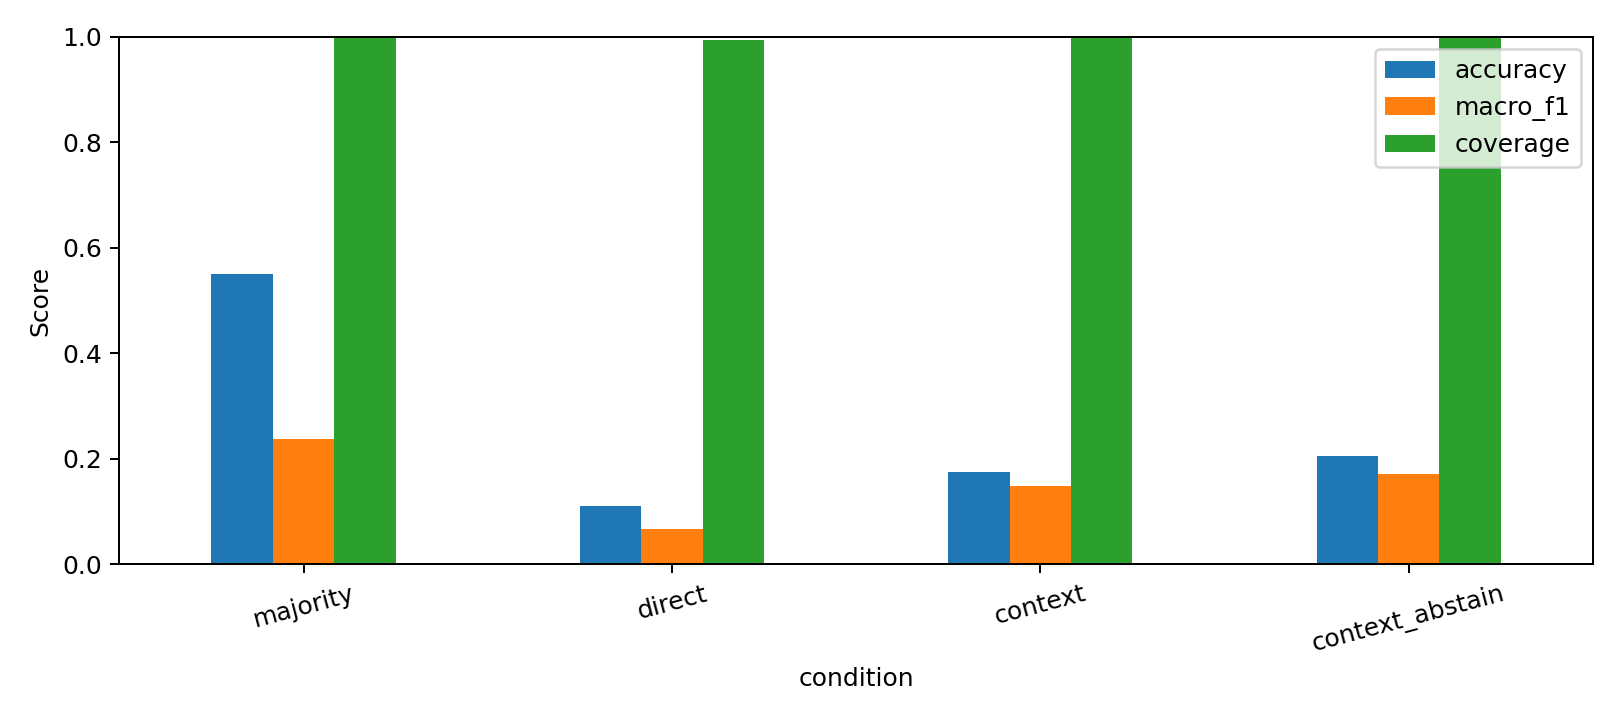
\includegraphics[width=0.69\textwidth]{condition_comparison.png}
\caption{Accuracy, macro-F1 and coverage exported by the original executed Colab notebook. Metrics are shown on the same scale for all four conditions.}
\label{fig:overview}
\end{figure*}

\subsection{Paired changes and comparison fairness}
Since the same PMIDs are used in every condition, it is possible to count which specific questions change correctness. Relative to direct prompting, supplied abstract context corrects 19 formerly incorrect decisions and makes six formerly correct decisions incorrect; 16 remain correct under both methods and 159 are incorrect under both. The net gain is therefore $19-6=13$ questions, or $13/200=6.5$ percentage points. Relative to the basic abstract condition, the abstention instruction makes nine previously wrong decisions correct and three previously correct decisions wrong, a net gain of six questions (3.0 percentage points). These are descriptive paired comparisons for this run, not evidence of a general causal or statistically significant gain.

\begin{table}[t]
\centering
\caption{Paired accuracy changes on identical test IDs.}
\label{tab:paired}
\resizebox{\columnwidth}{!}{%
\begin{tabular}{lrrr}
\toprule
Comparison (new vs. prior) & Gained & Lost & Net / 200 \\
\midrule
Abstract vs. question only & 19 & 6 & +6.5 pp \\
Abstract+abstain vs. abstract & 9 & 3 & +3.0 pp \\
Abstract+abstain vs. question only & 25 & 6 & +9.5 pp \\
\bottomrule
\end{tabular}}
\end{table}

\section{Classwise Failure Analysis}
The largest systematic failure is in the \texttt{no} class. Although the test set includes 68 \texttt{no} questions, no LLM condition predicts \texttt{no}. Thus, every model condition has exactly zero recall for that class. The majority predictor also never predicts \texttt{no} because it always chooses \texttt{yes}. These counts are not a minor rounding issue; they show an inability of the tested prompts and small checkpoint to represent all three labels in actual output.

The direct condition collapses almost completely to \texttt{maybe}, so it correctly classifies all 22 \texttt{maybe} cases but fails on every \texttt{yes} and \texttt{no} case. Context changes the predicted distribution: the model now produces 26 \texttt{yes} and 174 \texttt{maybe} predictions, of which 19 and 16 are respectively correct. The context+abstention condition produces 36 \texttt{yes} and 164 \texttt{maybe} predictions, of which 25 and 16 are correct. The improvement in aggregate agreement comes from recovering some \texttt{yes} cases, while \texttt{maybe} recall decreases from 100\% to 72.7\% and \texttt{no} recall stays at zero.

\begin{table}[t]
\centering
\caption{Class recall in percent from saved outputs.}
\label{tab:recall}
\begin{tabular}{lrrr}
\toprule
Condition & Yes & No & Maybe \\
\midrule
Majority & 100.0 & 0.0 & 0.0 \\
Question only & 0.0 & 0.0 & 100.0 \\
Abstract & 17.3 & 0.0 & 72.7 \\
Abstract + abstain & 22.7 & 0.0 & 72.7 \\
\bottomrule
\end{tabular}
\end{table}

These recall values in Table~\ref{tab:recall} demonstrate why a single average is not enough to diagnose the model. The direct classifier's \texttt{maybe} recall is superficially perfect, but its macro-F1 is only 0.0664. The abstract classifier improves the macro-F1 to 0.1476, yet most questions remain incorrectly labeled. The majority predictor has a still-higher macro-F1 of 0.2366 despite answering every non-\texttt{yes} instance incorrectly. The benchmark distribution in Table~\ref{tab:gold} is therefore essential context for interpreting improvements.

\begin{figure*}[t]
\centering
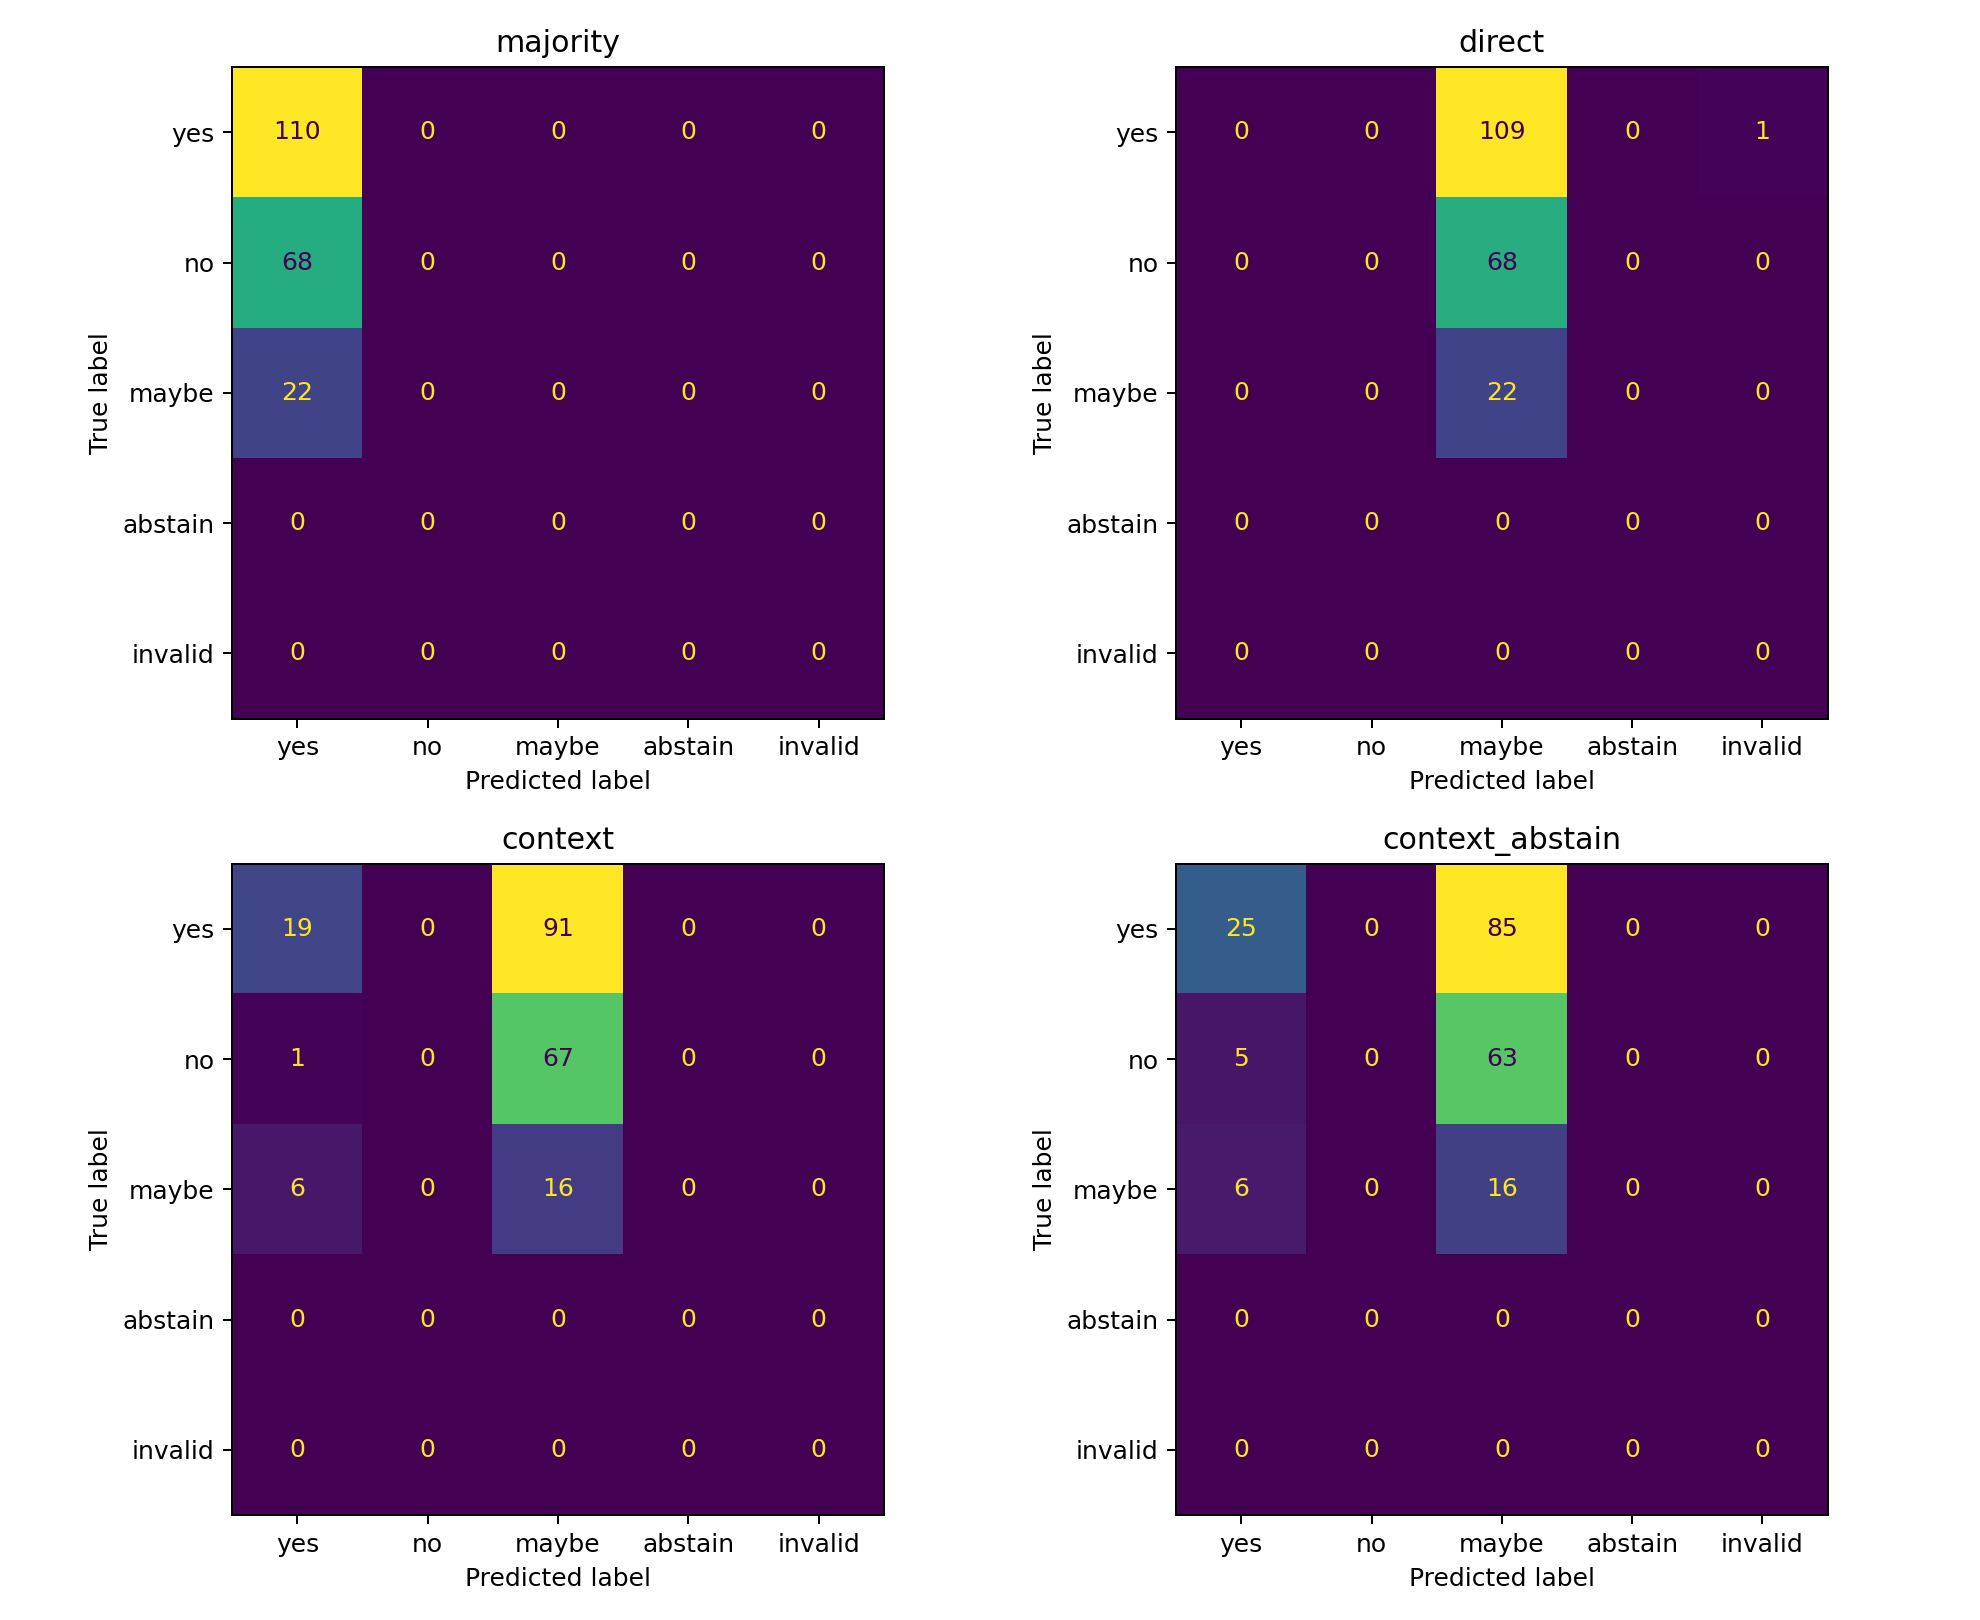
\includegraphics[width=0.69\textwidth]{confusion_matrices.png}
\caption{Archived per-condition confusion matrices. Columns for \texttt{abstain} and \texttt{invalid} expose formatting and selective-decision behavior rather than treating those outputs as benchmark labels.}
\label{fig:confusion}
\end{figure*}

The project archives the original confusion matrices in Fig.~\ref{fig:confusion}, a per-class metrics CSV, a list of incorrect examples with PMID identifiers, a paired-predictions CSV, and an additional paired-change summary independently derived from the saved rows. The item-level archive permits future error annotation without guessing which questions changed or silently altering the original measurements.

\section{Efficiency and Engineering Considerations}
In the recorded Colab run, mean batch-generation time per item was 14.46 ms for question-only prompting, 31.89 ms for supplied context, and 33.39 ms for the abstention prompt. Context conditions are slower under this measurement because their inputs are longer. These timings come from one machine and one session, are averaged from the recorded batches, and exclude several major parts of deployment latency. They are useful as relative diagnostics for the archived run, not hardware-independent performance claims.

The short generation limit of four new tokens simplifies constrained decision extraction and lowers computational cost. It also introduces a potential protocol restriction: a model that tends to explain its choice rather than immediately emit a label may be marked invalid. In this run, however, only one completion failed the parser, so format failures alone cannot explain the overall accuracy deficit. The dominant limitation is the distribution of otherwise syntactically valid class choices, especially the absence of \texttt{no} responses.

Reproducibility does not require shipping the approximately billion-byte model checkpoint inside the ZIP. Instead, the package contains the executed notebook, source identifier, dataset URL and hash, split PMIDs, version and hardware metadata, raw completions, scoring scripts, and original figures. The independent verifier works offline using Python's standard library. Repeating inference requires the external dataset and model download and may differ if the upstream model revision changes.

\section{Discussion and Threats to Validity}
The primary question has a narrow affirmative answer: for the recorded small checkpoint, test split and prompts, adding the associated abstract increased agreement with expert decisions. It does \emph{not} follow that the model learned or recovered correct biomedical reasoning. The manipulation changes both content and input length, and there is no length-matched irrelevant-abstract control. The evidence could help identify relevant studies, could alter how the prompt is parsed, or could trigger biases in the pretrained model. The current design does not separate those pathways.

The secondary question has a negative behavioral result. The instruction to \texttt{abstain} changed the model's class choices and improved agreement by three points over the basic context condition, but it produced no explicit withholding. Consequently, the experiment has no observed accuracy--coverage frontier. The \texttt{maybe} answers must not be retroactively interpreted as abstentions, because they are gold-standard labels and were explicitly permitted in all prompting conditions.

Several threats limit external interpretation. First, there is only one checkpoint, one development/test partition and one fixed prompt per condition. There are no independently rerun seeds or alternative model sizes. Second, the custom split and constrained decoding protocol are not identical to published PubMedQA benchmark evaluations. Third, the model revision is unavailable in recorded metadata, which obstructs bitwise replication. Fourth, public datasets may have appeared in a model's pretraining data; no contamination analysis was carried out. Fifth, label-level metrics do not inspect the truth of rationales, claims or citations. Finally, none of the task outputs have been reviewed as clinical recommendations, and no patient-level use is warranted.

The results also illustrate an important general methodological point from the preceding literature review: evaluation granularity must match the claim being made. The present work measures label agreement and output behavior; FActScore's atomic support, FELM's error annotation and ALCE's citation support would require different outputs and validation procedures. A paper about this experiment should not claim those properties on the basis of accuracy alone.

\section{Future Work and Reproducibility}
A first next experiment would compare matched abstract evidence with a randomly assigned \emph{length-matched irrelevant abstract}, while fixing the remaining prompt and generation settings. That would help distinguish evidence relevance from the effect of additional tokens. A second experiment would compare multiple prompt formats or appropriately sized model checkpoints on development examples, freeze the chosen setting, and evaluate on a new held-out set. Such work could investigate whether the missing \texttt{no} class reflects prompt sensitivity, model limitations, or another cause.

A third experiment would design an explicit selective-classification mechanism, such as a confidence threshold tuned only on development records, and then measure coverage and accuracy on unseen records. It should be reported separately from the prompt-only permission to abstain used here. Extending the problem to evidence citations or claim-level factuality would require an evidence retrieval and annotation stage, not only modified PubMedQA prompts.

For reproduction, the submission contains the exact executed notebook, a dependency record, dataset acquisition instructions, saved split IDs, all four prediction groups, and an offline verifier. Running \texttt{python verify\_results.py} recomputes the stored metrics without paid API access or downloading model weights. The Colab notebook can repeat model inference when a suitable runtime and public downloads are available. These are distinct levels of reproduction: \emph{metric audit} versus \emph{inference rerun}. The latter was not performed during final packaging.

\section{Conclusion}
On 200 held-out PubMedQA questions, matching abstract context improved a small instruction model's accuracy from 11.0\% to 17.5\%, and a prompt permitting abstention produced 20.5\% accuracy. These gains occurred within weak model baselines: the development-majority predictor reached 55.0\%, every model condition failed all \texttt{no} cases, and the supposed abstention option caused no abstentions. The negative and mixed findings are as important as the positive context difference, because they delimit precisely what the experiment established. Saving raw responses and independently auditing the scores makes this limited, resource-conscious study inspectable and reproducible while avoiding claims about unmeasured factuality dimensions.

\section*{AI Assistance and Accountability}
AI tools assisted the student's literature-to-experiment mapping, executable notebook workflow, evaluation auditing, documentation and manuscript drafting. The supplied executed Colab notebook and exported prediction ZIP are the evidence of model execution. Additional package analysis recomputed scores from these outputs; it did not run the GPU model again. No human review or instructor approval is claimed as complete. The student is responsible for checking, understanding and defending the submission.

\bibliographystyle{IEEEtran}
\bibliography{references}
\end{document}
